
\documentclass[preview]{standalone}

% pgfplots
\usepackage{pgfplots}
\pgfplotsset{compat=newest}
\usepackage{xcolor}
\usepackage{tikz-network}
\usepackage{graphicx}
\usepackage{float}
\usepackage{caption}
\usepackage{subcaption}
\usetikzlibrary{
    arrows.meta,
    matrix,
    positioning,
    patterns,
}
\begin{document}
\begin{figure}[h]
    \centering
    \begin{subfigure}[b]{0.45\textwidth}
        \centering
        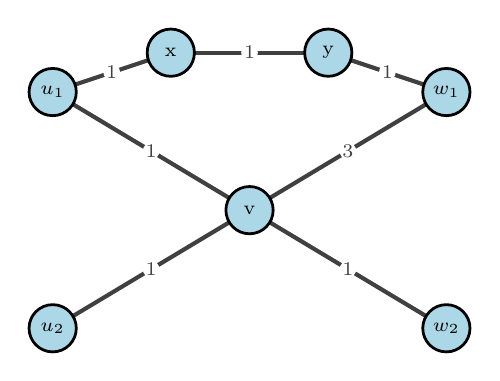
\begin{tikzpicture}
            \Vertex[x=0,y=0,label=v]{v}
            \Vertex[x=-2.5,y=1.5,label=$u_1$]{u1}
            \Vertex[x=-2.5,y=-1.5,label=$u_2$]{u2}
            \Vertex[x=-1,y=2,label=x]{x}
            \Vertex[x=1,y=2,label=y]{y}
            \Vertex[x=2.5,y=1.5,label=$w_1$]{w1}
            \Vertex[x=2.5,y=-1.5,label=$w_2$]{w2}
            \Edge[label=1](u1)(v)
            \Edge[label=1](u2)(v)
            \Edge[label=3](v)(w1)
            \Edge[label=1](v)(w2)
            \Edge[label=1](u1)(x)
            \Edge[label=1](x)(y)
            \Edge[label=1](y)(w1)
        \end{tikzpicture}
        \caption{Graph $G = (V,E)$}
    \end{subfigure}
    \begin{subfigure}[b]{0.45\textwidth}
        \centering
        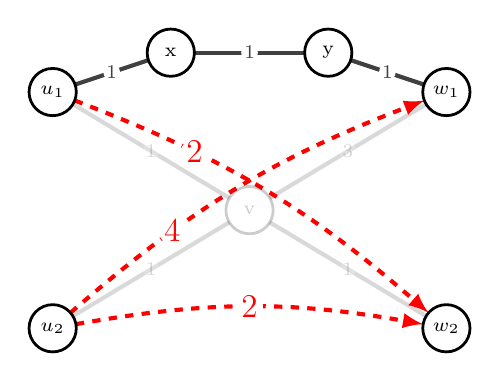
\begin{tikzpicture}
            \SetVertexStyle[TextOpacity=0.2,FillColor=white,LineOpacity=0.2]
            \Vertex[x=0,y=0,label=v,opacity=0.2]{v}
            \SetVertexStyle[TextOpacity=1,FillColor=white,LineOpacity=1]
            \Vertex[x=-2.5,y=1.5,label=$u_1$]{u1}
            \Vertex[x=-2.5,y=-1.5,label=$u_2$]{u2}
            \Vertex[x=-1,y=2,label=x]{x}
            \Vertex[x=1,y=2,label=y]{y}
            \Vertex[x=2.5,y=1.5,label=$w_1$]{w1}
            \Vertex[x=2.5,y=-1.5,label=$w_2$]{w2}
            \SetEdgeStyle[TextOpacity=0.2,TextFillOpacity=0.2,Opacity=0.2]
            \Edge[label=1](u1)(v)
            \Edge[label=1](u2)(v)
            \Edge[label=3](v)(w1)
            \Edge[label=1](v)(w2)
            \SetEdgeStyle[TextOpacity=1,TextFillOpacity=1,Opacity=1]
            \Edge[label=1](u1)(x)
            \Edge[label=1](x)(y)
            \Edge[label=1](y)(w1)
            \Edge[fontsize=\large,label=2,color=red,bend=10,Direct,style=dashed,distance=0.3](u1)(w2)
            \Edge[fontsize=\large,label=4,color=red,bend=10,Direct,style=dashed,distance=0.3](u2)(w1)
            \Edge[fontsize=\large,label=2,color=red,bend=10,Direct,style=dashed](u2)(w2)
        \end{tikzpicture}
        \caption{Graph $G' = (V', E')$ mit $V' = V - \{v\}$}
    \end{subfigure}
    \caption[Knotenkontraktion]{Beispiel einer Knotenkontraktion}
    \label{fig:ex_contraction}
\end{figure}
\end{document}